\section{Aufgabe 1}
    \subsection{a)}
        \subsubsection{}
            $$\text{Nullstellen von }f(x) = x^6 - x^2 \text{ in Wolframalpha: }$$
            \begin{center}
                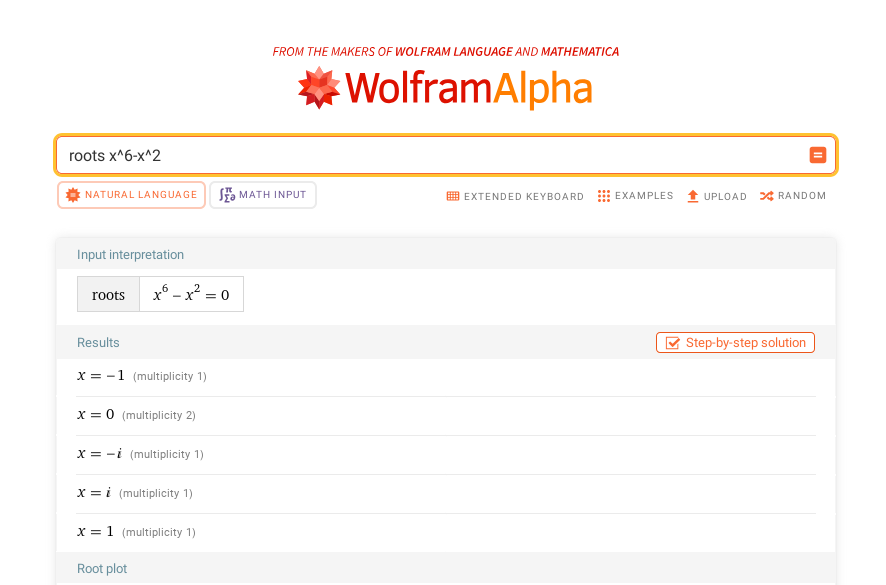
\includegraphics[width = 0.75\textwidth]{Aufgaben/01/1a)i).png}    
            \end{center}

        \subsubsection{}
            $$\text{Nullstellen von }f(x) = x^3 + 4x^2 - 7x + 2 \text{ in Wolframalpha: }$$
            \begin{center}
                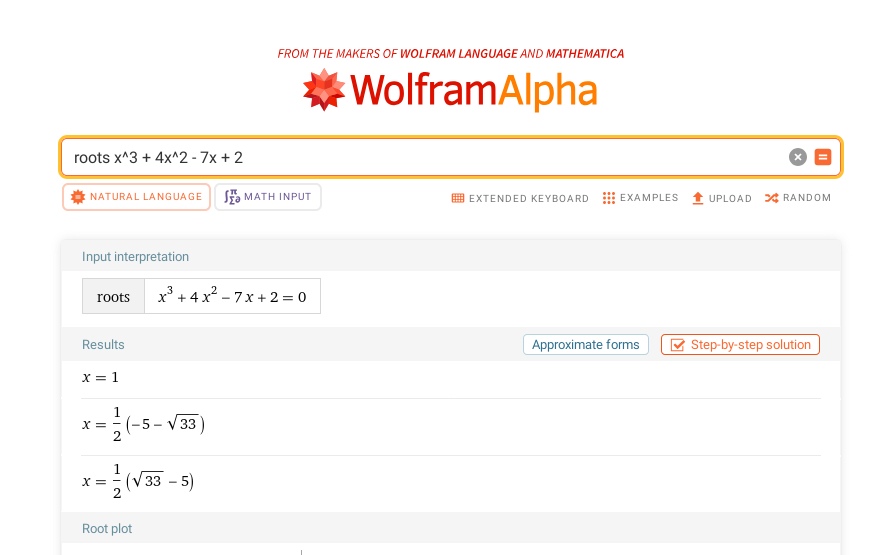
\includegraphics[width = 0.75\textwidth]{Aufgaben/01/1a)ii).png}    
            \end{center}
    \subsection{b)}
        $$\text{Potenzreihe von }a^x \text{ für } a>0, a\in \mathbb{R} \text{ in Wolframalpha: }$$
            \begin{center}
                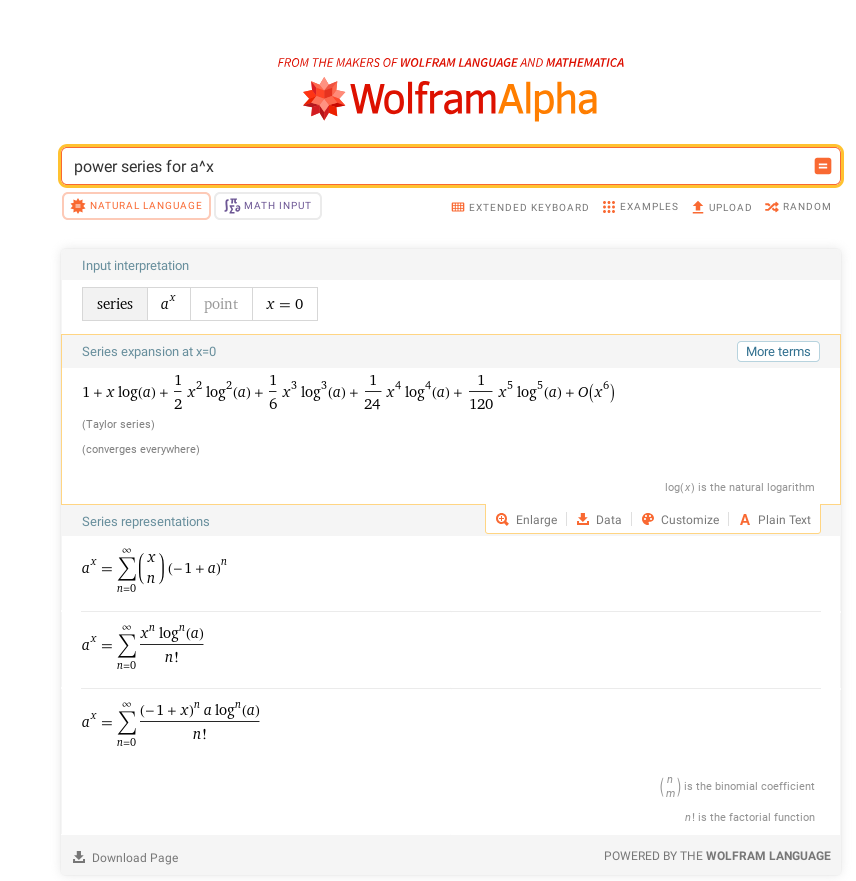
\includegraphics[width = 0.75\textwidth]{Aufgaben/01/1b).png}    
            \end{center}

        Da diese Potenzreihe für alle $a \in \mathbb{R}$ gilt, gilt diese analog auch für $a>0$

            